\chapter{Obesity associated genetic signatures and cancer}
\label{cha:obesity_genetic_signatures_and_cancer}

The obesity associated genetic signatures are central to this project in order to clarify the relationship between \gls{bmi} and cancer.
Firstly in this chapter, the previously identified obesity associated signatures from the studies conducted by \citet{Creighton2012} and \citet{Fuentes-Mattei2014} were examined in turn to judge the agreement of these signatures with the sample \gls{bmi}/\gls{bmi} status, as presented in thier results.
Secondly, novel obesity associated genetic signatures were identified in the Creighton \textit{et al.} (CR) data set and was compared with the signatures from the Creighton \textit{et al.} and Fuentes-Mattei \textit{et al.} studies.
Lastly, the presence of common genes or pathways that were associated with obesity in multiple types of cancer was explored using the \gls{icgc} cancer data sets.

\section{Obesity associated genetic signature from \citet{Creighton2012} study}
\label{sec:creighton_obesity_metagene}

Obesity metagene was created using the obesity associated genetic signatures from the \citet{Creighton2012} study.
There was no description about the normalisation method used by Creighton \textit{et al.} when they first analysed their data, so the more reliable \gls{rma} method was used to  normalise the CR data set.
The obesity metagene was plotted in a heatmap with the sample gene expression  to check whether the metagene scores were in accordance with the overall gene expression of the samples (\cref{fig:crmetaheat}).

\begin{figure}[htb]
	\centering
	\includegraphics[page=3,width=0.8\linewidth]{results1/creighton_mg_heatmap1}
	\caption[Obesity metagene from \citet{Creighton2012} study and sample gene expression in CR data]{Heatmap showing the obesity metagene from the \citet{Creighton2012} study with the gene expressions of obesity associated genes in CR data.
	Level of expression is represented in the top right histogram, where low and high gene expression were colour-coded with blue and red, respectively.
	Each row of the heatmap represents a gene from the obesity associated genetic signature, and each column of the heatmap represents a sample from CR data.
	The obesity associated metagene scores of the samples are shown in a separate row at top of the heatmap, and the tree diagram of the heirarchical clustering of the genes is shown to the left of the heatmap.
	For clarity, the metagene scores were flipped in order to match the results from the \citet{Creighton2012} study.}
	\label{fig:crmetaheat}
\end{figure}

As shown in \cref{fig:crmetaheat}, high obesity associated metagene score of the sample reflected low expression in majority of the genes in the signature, and in contrast, low obesity associated metagene score of the sample reflected high expression in majority of the genes in the signature.
This was consistent with the reported property of the obesity associated signature by \citet{Creighton2012} (see \cref{ssub:creighton_study}).
To provide further evidence that the obesity associated metagenes were in fact associated with the \gls{bmi} status and \gls{bmi} value of the samples, a box plot and a scatter plot were created, respectively (\cref{fig:crmetaboxplot}).

\begin{figure}[htp!]
	\centering
	\includegraphics[page=4,width=0.45\linewidth]{results1/creighton_mg_heatmap1}
	\hfill
	\includegraphics[page=5,width=0.45\linewidth]{results1/creighton_mg_heatmap1}
	\caption[Obesity metagene from the \citet{Creighton2012} study and sample \gls{bmi}/\gls{bmi} status in CR data]{Box plot and scatter plot showing the association of the obesity metagene from the \citet{Creighton2012} study with sample \gls{bmi} status and \gls{bmi} from CR data, respectively.
	In the box plot, the p-values above the groups represent the statistical significance of the association of the metagene with the overweight or obese group compared with the normal weight group.
	The \gls{anova} p-value shows the statistical significance of the association of the metagene with the sample \gls{bmi} groups.
	In the scatter plot, $R^2$- and p-values describe the adjusted coefficient of determination of the regression line and the statistical significance of the linear model used to draw the regression line, respectively.}
	\label{fig:crmetaboxplot}
\end{figure}

\cref{fig:crmetaboxplot} clearly showed that the obesity metagene from the \citet{Creighton2012} study significantly associated with the sample \gls{bmi} status, as well as sample \gls{bmi} value (include p-value and r-squared).
It should be noted here that the obesity associated metagene significantly associated with the samples that were obese, but not with the samples that were overweight.
This was due to the fact that the obesity associated genetic signatures were originally identified from the comparison of the samples that were obese with the samples that were not obese, and therefore the metagene scores were significant with the obese group, but not with the overweight group.
In addition to this, although the regression line in the scatter plot showed statistically significant association with sample \gls{bmi}, the sample \gls{bmi} values seemed to be randomly dispersed across the metagene scores.
This suggested that perhaps the obesity metagene from the \citet{Creighton2012} study was not associated with sample \gls{bmi} as strongly as expected.
\\

\noindent
Now that the association of the obesity metagene from the \citet{Creighton2012} study was established in CR data set, the obesity associated signature was generated in the \gls{icgc} cancer data.
The direction of the obesity associated metagene was checked in the CR data first, so that high metagene scores reflected high sample \gls{bmi} and low metagene scores reflected low sample \gls{bmi} (\cref{fig:crmetaboxplot}).
The transformation matrix was then created in CR data, as described in \cref{sub:svd}.

All of the \gls{icgc} data were normalised as described in \cref{ssub:rna_seq_data}.
Before the transformation matrix was applied to the log$_{10}$-normalised cancer data, the suitability of standardised data or untouched (non-standardised) data was determined (see \cref{sec:metagenes_created_from_raw_data_vs_standardised_data_icgc}).
From these results, the standardised data was found to be the most suitable to use for matrix transformation.
The transformation matrix was applied to each cancer data set in turn to obtain the Creighton \textit{et al.} obesity metagenes from each of the data set.
Each obesity metagenes were plotted in a heatmap with the corresponding data set in which the metagene was taken from (\cref{fig:crmetaicgc}; \cref{sec:rest_of_the_icgc_cancer_heatmap_resutls}).
These heatmaps confirmed that the obesity associated metagene derived from CR data was able to capture the overall gene expression pattern, where the metagene scores reflected the expression levels of majority of the genes in the signature.
As before, association of the obesity metagene with the sample \gls{bmi} and \gls{bmi} status was checked in their respective cancer data set (\cref{fig:crmetaicgc}; \cref{sec:rest_of_the_icgc_cancer_heatmap_resutls}).
Out of all the cancer types, only \gls{blca} data set showed significant association of obesity metagene with the overweight group (but not with the obese group).
However, neither the \gls{anova} p-value nor the regression line in the scatter plot were statistically significant, suggesting that this apparent association with the overweight group was not due to the obesity metagene (?).

\begin{figure}[htp!]
	\centering
	\includegraphics[page=3,width=0.8\linewidth]{results1/crtcga_std}\\
	\vspace{1em}
	\includegraphics[page=4,width=0.45\linewidth]{results1/crtcga_std}
	\hfill
	\includegraphics[page=5,width=0.45\linewidth]{results1/crtcga_std}
	\caption[Obesity metagene from the \citet{Creighton2012} study in \acrshort{icgc} \acrshort{blca} data]{Heatmap, box plot and scatter plot showing the association of obesity metagene from the \citet{Creighton2012} study with sample gene expression, \gls{bmi} and \gls{bmi} status from \gls{icgc} \gls{blca} data, respectively.
	The results for other cancer types are in \cref{app:a}.
	Scales, p-values and $R^2$-value are as described in previous figures.}
	\label{fig:crmetaicgc}
\end{figure}

There could be several reasons for the apparent lack of association of the metagene with sample \gls{bmi}/\gls{bmi} status.
First, transformation matrix was derived from CR microarray data, but the \gls{icgc} cancer data were \gls{rnaseq} data.
Though the log$_{10}$ normalisation and standardisation of the data was the most appropriate adjustment to be made to the \gls{rnaseq} data, this adjustment was not equivalent to the \gls{rma} normalisation method that was used on the microarray data.
Secondly, none of the \gls{icgc} cancer originated from breast as in CR data.
Since the obesity associated signature was identified in breast cancer data, the signature may be specific to breast cancer and may not be suitable in other cancer types.
\\

\noindent
To check whether the metagene was specific to breast cancer microarray data, the same transformation matrix was applied to the \gls{nzbc} microarray data from \citet{Print2016} study (referred to as \gls{nzbc} data hereafter).
\gls{nzbc} data was normalised with \gls{rma} method and the transformation matrix was applied to the normalised data to obtain the metagene.
The metagene was again compared with the gene expression of the samples with a heatmap and the association of the metagene with the sample \gls{bmi}/\gls{bmi} status was examined with box and scatter plots (\cref{fig:crmetaprint}).

The obesity metagene managed to reflect the overall gene expression of the samples in \gls{nzbc} data.
However, as with \gls{icgc} cancer data, the obesity metagene scores did not significantly associate with the sample \gls{bmi} or \gls{bmi} status.
These results confirmed that the lack of association of the obesity metagene from CR data was not due to the technology in which the data was gathered (mcroarray or \gls{rnaseq}), nor the cancer type in which the transformation matrix was applied to.

\begin{figure}[htp!]
	\centering
	\includegraphics[width=0.8\linewidth,page=3]{results1/cris_cr_trans_meta}\\
	\vspace{1em}
	\includegraphics[width=0.45\linewidth,page=4]{results1/cris_cr_trans_meta}
	\hfill
	\includegraphics[width=0.45\linewidth,page=5]{results1/cris_cr_trans_meta}
	\caption[Obesity metagene from \citet{Creighton2012} study in \gls{nzbc} data]{Heatmap, box plot and scatter plot showing the association of obesity metagene from the \citet{Creighton2012} study with sample gene expression, \gls{bmi} and \gls{bmi} status from \gls{nzbc} data, respectively.
	Scales, p-values and $R^2$-value are as described in previous figures.}
	\label{fig:crmetaprint}
\end{figure}

All together, all of these results suggest that the obesity metagene identified in the study conducted by \citet{Creighton2012} associated with sample \gls{bmi} and \gls{bmi} status only in CR data.
The lack of association with \gls{bmi} was not due to the type of technology platform in which the data was gathered, as neither the \gls{icgc} \gls{rnaseq} data nor \gls{nzbc} microarray data showed no significant association with the obesity metagene.
Furthermore, the obesity metagene was not dependent on the cancer type since the obesity associated genetic signature did not show significant association in neither the \gls{icgc} cancer data nor in \gls{nzbc} data.

One possible reason why the obesity metagene from the \citet{Creighton2012} study did not show significant association with other data sets could be because the genetic signature was in fact not an obesity specific signature, but a signature that was detected due to another clinical variable.
Another reason for this apparent lack of association could be that the genetic signature was too specific to the data and was not a broad obesity associated genetic signature, but an obesity associated signature specifically for CR data set.

\section{Obesity associated genetic signature from \citet{Fuentes-Mattei2014} study}
\label{sec:fm_obesity_metagene}

Since the obesity associated genetic signature from the \citet{Creighton2012} study was not associated with sample \gls{bmi} or \gls{bmi} status in other data sets, the obesity associated genetic signature from the \citet{Fuentes-Mattei2014} study (FM) was examined to see whether FM obesity metagene associated with sample \gls{bmi} or \gls{bmi} status.
Since FM data set did not have sample \gls{bmi} information, FM obesity metagene was not able to be compared with the sample \gls{bmi} or \gls{bmi} status in the original FM data.
However, the transformation matrix was still applied to other cancer data to see whether FM obesity metagene associated with sample \gls{bmi}/\gls{bmi} status

Firstly, FM data was normalised with the \gls{rma} method and \gls{svd} was applied to the normalised FM data to get the transformation matrix.
The transformation matrix was used to transform the \gls{rma}-normalised CR data to extract FM obesity metagene scores in CR data.
FM obesity metagene scores were compared with gene expressions and sample \gls{bmi}/\gls{bmi} status in CR data, as shown in \cref{fig:fmmetacr}.
Clearly, like with the obesity metagene identified by Creighton \textit{et al.}, FM obesity metagene was reflective of the overall gene expression of the samples, but did not associate with the sample \gls{bmi} or \gls{bmi} status.

\begin{figure}[htp!]
	\centering
	\includegraphics[page=3,width=0.8\linewidth]{results1/cr_fm_meta}\\
	\vspace{1em}
	\includegraphics[page=4,width=0.45\linewidth]{results1/cr_fm_meta}
	\hfill
	\includegraphics[page=5,width=0.45\linewidth]{results1/cr_fm_meta}
	\caption[FM metagene in CR data]{Heatmap, box plot and scatter plot showing the association of FM obesity associated metagene with sample gene expression, \gls{bmi} and \gls{bmi} status from CR  data, respectively.
	Scales, p-values and $R^2$-value are as described in previous figures.}
	\label{fig:fmmetacr}
\end{figure}

Next, the transformation matrix was applied to the \gls{icgc} cancer data and resulting metagenes were compared with the gene expression and sample \gls{bmi}/\gls{bmi} status.
As evident in \cref{fig:fmmetaicgc}, FM obesity metagene scores appeared to reflect the overall gene expression of FM obesity associated genetic signature.
As with all the results in this chapter so far, FM obesity metagene did not significantly associate with any of the \gls{icgc} cancer data, except in \gls{blca} data set (\cref{fig:fmmetaicgc}).
FM obesity metagene significantly associated with the overweight group (but not with the obese group), and also had a significant \gls{anova} p-value.
On the contrary to the association of the metagene with the sample \gls{bmi} status, FM obesity metagene was not associated with sample \gls{bmi}.
These results suggested that the samples that were overweight in the \gls{blca} data set had similar biological properties as the samples that were obese in FM data set.
However, due to the fact that FM metagene lacked association with sample \gls{bmi} in \gls{blca} data set and that the metagene did not show any significant association in any other cancer type, it was difficult to determine whether the observed association of FM obesity metagene with the overweight group of samples was truly reflective of the effect resulted from FM metagene.
Lastly, the transformation matrix was applied to \gls{nzbc} data (\cref{fig:fmmetacris}).
Again, FM obesity metagene scores reflected the gene expression of the samples, did not significantly associate with sample \gls{bmi}/\gls{bmi} status.
\\

\begin{figure}[htp!]
	\centering
	\includegraphics[page=3,width=0.8\linewidth]{results1/fm_meta_ICGC}\\
	\vspace{1em}
	\includegraphics[page=4,width=0.45\linewidth]{results1/fm_meta_ICGC}
	\hfill
	\includegraphics[page=5,width=0.45\linewidth]{results1/fm_meta_ICGC}
	\caption[FM metagene in \acrshort{icgc} \acrshort{blca} data]{Heatmap, box plot and scatter plot showing the association of FM obesity associated metagene with sample gene expression, \gls{bmi} and \gls{bmi} status from \acrshort{icgc} \acrshort{blca} data, respectively.
	The results for other cancer types are in \cref{app:a}.
	Scales, p-values and $R^2$-value are as described in previous figures.}
	\label{fig:fmmetaicgc}
\end{figure}

\begin{figure}[htp!]
	\centering
	\includegraphics[page=3,width=0.8\linewidth]{results1/cris_fm_meta}\\
	\vspace{1em}
	\includegraphics[page=4,width=0.45\linewidth]{results1/cris_fm_meta}
	\hfill
	\includegraphics[page=5,width=0.45\linewidth]{results1/cris_fm_meta}
	\caption[FM metagene in \gls{nzbc} data]{Heatmap, box plot and scatter plot showing the association of FM obesity associated metagene with sample gene expression, \gls{bmi} and \gls{bmi} status from \gls{nzbc} data, respectively.
	Scales, p-values and $R^2$-value are as described in previous figures.}
	\label{fig:fmmetacris}
\end{figure}

\noindent
These results showed that FM obesity associated metagene was not transferable to other cancer data sets, similar to the obesity metagene identified by Creighton \textit{et al.}.
This meant that both the obesity metagenes identified by Creighton \textit{et al.} and Fuentes-Mattei \textit{et al.} may have been too specific to the orignial data set in which the signatures were identified in.
Furthermore, there was a possibility that these obesity associated metagenes were not related to obesity, but associated with a different clinical variable that may be closely related to \gls{bmi}.

\section{Novel obesity associated genetic signatures from \citet{Creighton2012} data set}
\label{sec:creighton_obesity_metagene_new}

\subsection{Identification of obesity associated genetic signatures}
\label{sub:identification_of_obesity_associated_genetic_signatures}

Both the obesity associated metagenes generated from CR data and FM data were able to capture the overall pattern of gene expression of the genetic signature in the samples, but did not associate with sample \gls{bmi}/\gls{bmi} status.
One possible reason for this result could be that the obesity associated genetic signatures from the \citet{Creighton2012} and \citet{Fuente-Matter2014} studies may not have been truly associated with sample \gls{bmi}  status, but with another clinical variable.
To reject this possibility, obesity associated genetic signatures were identified in CR data after controlling for all the clinical variables in the data set.
FM data set was not used to get obesity associated genetic signatures, as no \gls{bmi} information was available for the samples in FM data.

Firstly, to validate whether the identified obesity associated genetic signature was similar to the signature that Creighton \textit{et al.} had originally found, the identified \glspl{deg} were compared with the original genetic signature identified by Creighton \textit{et al.}.
\glspl{deg}  were identified between the samples from obese patient and non-obese patient in the \gls{rma}-normalised CR data, as described in \cref{sec:gene_expression_analysis}.
Without adjusting the p-value with FDR, 5278 gene probes and 1781 gene probes were significant at p \textless{} 0.05 and p \textless{} 0.01, respectively.
After afjustment, there were only 9 gene probes significant at p \textless{} 0.05 and no gene was significant at p \textless{} 0.01.
Furthermore, there were only 61 gene probes that were significantly differentially expressed at p \textless{} 0.05 with a log$_2$ \gls{fc} greater than 1.2.
From these observations, the log$_2$ fold change of the gene probes were ignored and the threshold p-value was set to 0.01 (without adjustment) for the identification of gene probes.
This was to include as many gene probes as possible without losing power (?).
Additionally, when there were more than 799 gene probes identified, only the most significant 799 gene probes were taken as the obesity associated genetic signature, as this many genes were originally identified by Creighton \textit{et al.}.
These criteria were applied for the identification of other genetic signatures as well.

The above analysis was repeated with the residual data (\gls{rma}-normalised CR data that had been controlled for other clinical variables; see \cref{sub:residual_data_creation}).
The clinical variables controlled were age, ethnicity, menopause status, tumour grade, hormone (\gls{er}, \gls{pr}, and \gls{her2}) statuses  and \gls{ln} status.
In the residual data, 1104 gene probes were significant with unadjusted p-value (p \textless{} 0.01).
Again, the most significant 799 genes were taken as the obesity associated genetic signature from this data.

In addition to the above two obesity associated genetic signatures, two more sets of genetic signatures were identified by taking the common genes between the above two signatures with the original obesity associated genetic signatures.
There were 239 common gene probes between the original genetic signature and the gene probes identified from the unadjusted CR data, and 168 common gene probes between the original signature and gene probes from residual data in CR data.
The genetic signatures identified were summarised as a Venn diagram, as shown in \cref{fig:venn1}.
\\

\begin{figure}[htp!]
	\centering
	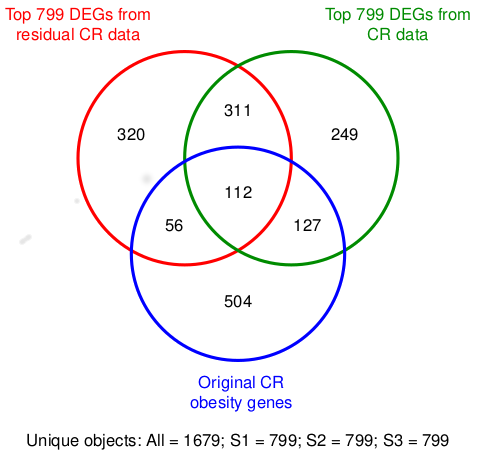
\includegraphics[width=0.5\linewidth]{results1/deg_venn1}
	\caption[Veen diagram of the \glspl{deg} identified from CR data (all samples)]{Venn diagram showing the common genes between the signatures obtained from unadjusted and clinical variable-adjusted CR data and the original obesity associated genetic signature.}
	\label{fig:venn1}
\end{figure}

\noindent
There was a possible bias between different ethnic groups, where African American patients were more likely to be obese compared to the Caucasian patients (see \cref{ssub:creighton_study}).
Though ethnicity was controlled in the residual data, the effect of ethnicity on the data was completely removed to prevent any possibility of ethnicity influencing the analysis.
Therefore, the effect of ethnicity was completely removed by considering only the Caucasian patients in CR data, which left a total of 77 Caucasian patients in the data set.
With this Caucasian-only data set, obesity associated genetic signatures were identified as described above; first with unadjusted data, then with the data with clinical variables adjusted (except ethnicity, as it has already been controlled for by considering Caucasian samples only), and lastly the common genes with the original signature were identified.

2129 and 1558 gene probes were identified in the unadjusted and clinical variable-adjusted Caucasian patient data, respectively.
As before, the most significant 799 gene probes were selected from these gene probes.
There were 148 and 92 common gene probes with the original genetic signatures and unadjusted or clinical variable-adjusted Caucasian patient data set, respectively.
Again, Venn diagram was used to summarise the genes identified from the Caucasian patient data set (\cref{fig:venn2}).
\\

\begin{figure}[htp!]
	\centering
	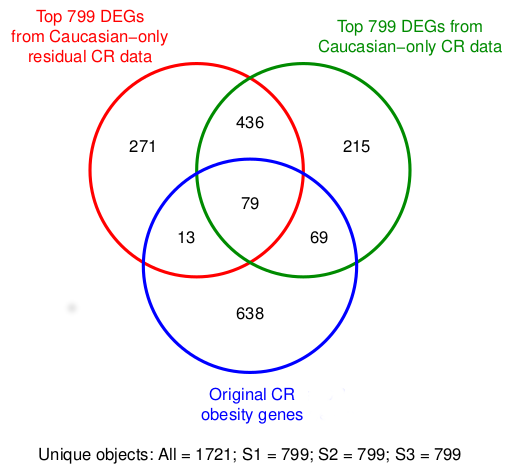
\includegraphics[width=0.5\linewidth]{results1/deg_venn2}
	\caption[Summary of the \glspl{deg} identified from CR data (Caucasian patient data)]{Venn diagram showing the common genes between the signatures obtained from unadjusted and clinical variable-adjusted CR data (Caucasian patients only) and the original obesity associated genetic signature.}
	\label{fig:venn2}
\end{figure}

\noindent
In addition to these eight obesity associated genetic signatures, a genetic signature was identified based on the correlation of gene probe expression with sample \gls{bmi} as continuous values, rather than discrete values as in \gls{bmi} status.
However, no significant genes were identified and thus was not used for further analysis (results detailed in appendix).

All of these obesity associated genetic signatures (eight in total) were checked to see whether these signatures had significant association with sample \gls{bmi}/\gls{bmi} status in various data set.
For simplicity, the abbreviations in \cref{tab:mg_abbrev} will be used to refer to the appropriate genetic signatures.

\begin{table}[htpb]
	\centering
	\caption{Summary of the abbreviations used to refer to the different obesity associated genetic signatures}
	\label{tab:mg_abbrev}
	\begin{tabular}{lp{0.51\textwidth}c}
		\hline
		\hline
		Abbreviation & Definition & No. of gene probes\\
		\hline
		\rule{0pt}{2.25ex}Or      & Original obesity associated genetic signature identified by \citet{Creighton2012}                       & 799\\
		\rule{0pt}{2.25ex}Cr      & Obesity associated genetic signature identified from unadjusted CR data                                & 799 \\
		\rule{0pt}{2.25ex}CrOl    & Genes common between Or and Cr genetic signatures                                                       & 239\\
		\rule{0pt}{2.25ex}Res     & Obesity associated genetic signature identified from clinical variable-adjusted CR data                & 799\\
		\rule{0pt}{2.25ex}ResOl   & Genes common between Or and Res genetic signatures                                                      & 168\\
		\rule{0pt}{2.25ex}Ca      & Obesity associated genetic signature identified from unadjusted Caucasian-only CR data                 & 799\\
		\rule{0pt}{2.25ex}CaOl    & Genes common between Or and Ca genetic signatures                                                       & 148\\
		\rule{0pt}{2.25ex}CaRes   & Obesity associated genetic signature identified from clinical variable-adjusted Caucasian-only CR data & 799\\
		\rule{0pt}{2.25ex}CaResOl & Genes common between Or and CaRes genetic signatures                                                    & 92\\
		\hline
		\hline
	\end{tabular}
\end{table}

\subsection{Novel obesity associated signatures and sample \gls{bmi}/\gls{bmi} status}
\label{sub:_novel_obesity_associated_signatures_and_sample_bmi}

As with the Or signature, all eight obesity associated genetic signatures were validated in CR data set first, and then compared in other cancer data sets by using the transformation matrix generated in CR data.
% Before the metagenes were created, all of the signatures were converted into gene symbols, as described in \cref{sec:data} (\cref{tab:signature_gene_num}).
CR data (unadjusted, all samples included) was normalised with \gls{rma} method and \gls{svd} was applied to generate the metagene for the corresponding genetic signature.
The direction of the metagenes were first examined to make sure that all of the metagenes were in line with one another (see \cref{sub:metagene_direction}; results shown in appendix).
The comparison of the metagenes with the sample gene expression in CR data were displayed as heatmaps (\cref{fig:degmetacr}).
It was clear from the heatmaps that all of the metagenes reflected the overall expression of the corresponding genetic signatures.
The association of the metagenes with sample \gls{bmi}/\gls{bmi} status was significant for all eight of the metagenes identified (\cref{fig:degmetacr}).
These results confirmed that all of the obesity associated genetic signatures identified in \cref{sub:identification_of_obesity_associated_genetic_signatures} significantly associated with sample \gls{bmi}/\gls{bmi} status in CR data, where the metagenes were derived from.

\begin{figure}[htp!]
	\centering
	\includegraphics[page=3,width=0.8\linewidth]{results1/cr_deg_meta_vs_clin}\\
	\vspace{1em}
	\includegraphics[page=4,width=0.45\linewidth]{results1/cr_deg_meta_vs_clin}
	\hfill
	\includegraphics[page=5,width=0.45\linewidth]{results1/cr_deg_meta_vs_clin}
	\caption[Cr obesity associated metagene in CR data]{Heatmap, box plot and scatter plot showing the association of Cr obesity associated metagene with sample gene expression, \gls{bmi} and \gls{bmi} status from CR data, respectively.
	The results for other metagenes are in \cref{app:a}.
	Scales, p-values and $R^2$-value are as described in previous figures.}
	\label{fig:degmetacr}
\end{figure}

Additionally, the correlation of all of the obesity associated metagenes were examined to see whether these metagenes were similar to one another.
As clearly shown in \cref{fig:cr_meta_cor}, there were two distinct groups within the eight metagenes; the first group contained the metagenes that were not overlapped with the Or metagene (Cr, Res, Ca and CaRes), while the other group had the overlapped metagenes (CrOl, ResOl, CaOl and CaResOl).
With that said, all eight metagenes showed high correlation with one another (lowest correlation approximately at 0.85), which suggested that all of these metagenes were detecting similar underlying biological mechanism from the data.

\begin{figure}[htpb]
	\centering
	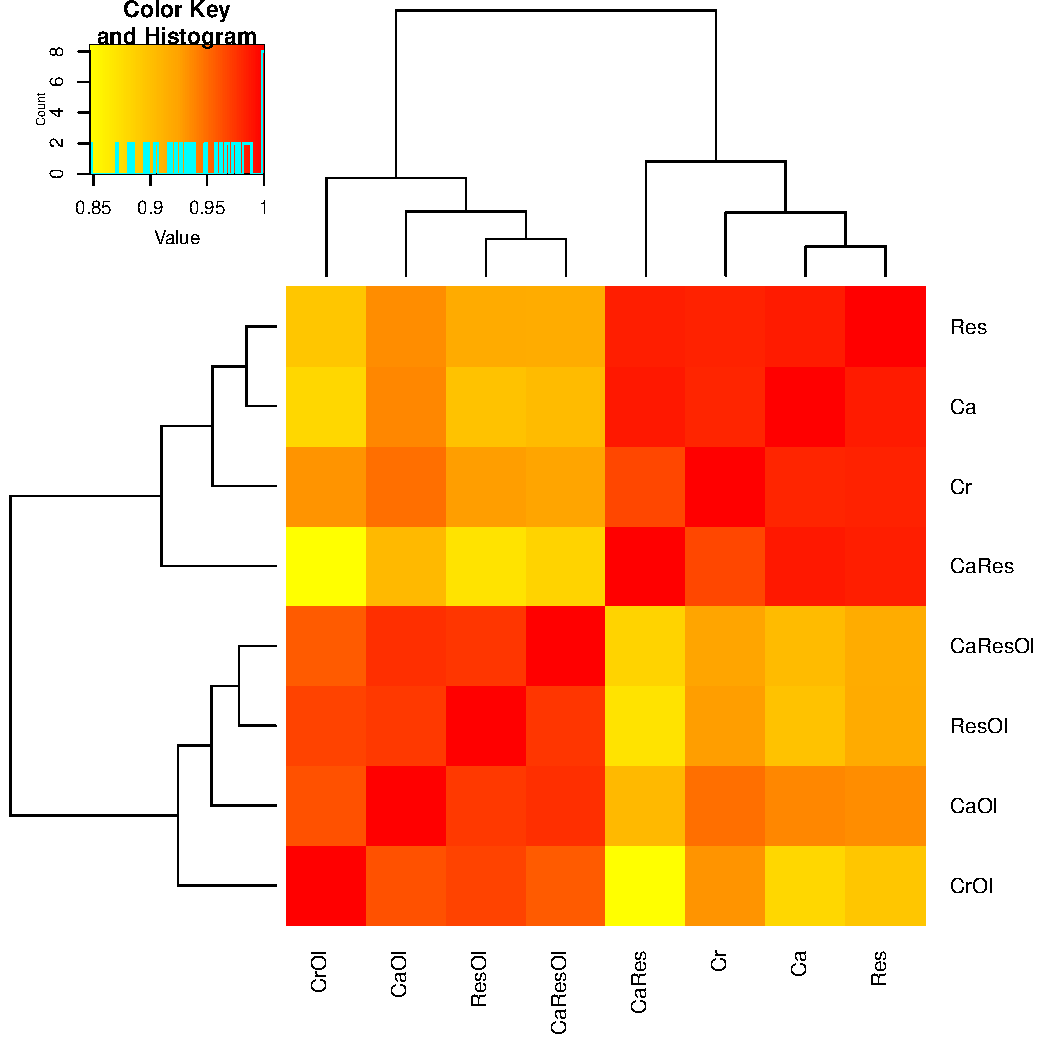
\includegraphics[width=0.8\linewidth]{results1/cr_meta_cor}
	\caption[Pearson correlation of all eight obesity associated metagenes identified in CR data]{Heatmap showing the Pearson correlation of all eight obesity associated metagenes from CR data with one another.
	\gls{svd} was applied to \gls{rma}-normalised CR data to generate each of the eight metagenes.
	High and low correlation were represented as red and blue, respectively, where the colours were matched with the values on the scale shown in top right.}
	\label{fig:cr_meta_cor}
\end{figure}

To confirm whether these metagenes showed significant association with sample \gls{bmi}/\gls{bmi} status in other cancer data sets, transformation matrix was applied to the \gls{icgc} cancer data and \gls{nzbc} data.
Firstly in \gls{icgc} cancer data sets, all eight metagene scores were reflective of the sample gene expression of the genetic signatures (\cref{fig:degmetaicgc}).
In all cancer types but \gls{blca}, none of the metagenes significantly associated with the sample \gls{bmi}/\gls{bmi} status (results shown in \cref{app:a}).
As shown in \cref{fig:degmetaicgc}, only the \gls{blca} data set showed significant association of the Cr metagene with sample \gls{bmi}/\gls{bmi} status.
With the metagenes other than Cr metagene, Res, CrOl and Ca metagenes showed statistical significance in overweight group, \gls{anova} and the regression line p-values; CaRes metagene was significant in overweight group and \gls{anova} p-value; CrOl and ResOl metagenes were significant in overweight group; and ResOl and CaOl metagenes were not significant in \gls{blca} data set.

This was unexpected since all of the genetic signatures were results of gene expression analysis between the non-obese group and the obese group of samples in CR data, and yet the metagenes showed significant association with the overweight group in \gls{blca} data set.
These results suggested that the samples that were overweight in \gls{blca} data were similar in phenotype with the samples that were obese in CR data.
Again, due to the fact that all of the metagenes lacked association with sample \gls{bmi}/\gls{bmi} status in all other \gls{icgc} data set, it was difficult to conclude whether the observed association of many of the obesity metagenes with the overweight group of samples was truly reflective of the effect resulted from these metagenes.

\begin{table}[htpb]
	\centering
	\caption{Statistics of all the obesity metagenes in \gls{blca} cancer data}
	\label{tab:degmetablca}
	\begin{threeparttable}
		\begin{tabular}{lccccc}
			& \multicolumn{3}{c}{ P-values} & \multicolumn{2}{c}{ Regression line statistics}\\
			\cmidrule(r){2-4} \cmidrule(r){5-6}
			 Metagenes &  Overweight &  Obese &  \gls{anova} &  R$^2$ &  P \\
			\hline
			\hline
			\rule{0pt}{2.25ex}Cr & {\bfseries 0.0134}\tnote{1} & 0.1365 & {\bfseries 0.0387} & 0.0171 & {\bfseries 0.0195} \\
			Res                  & {\bfseries 0.0055}          & 0.1974 & {\bfseries 0.0196} & 0.0117 & {\bfseries 0.0446} \\
			CrOl                 & {\bfseries 0.0383}          & 0.4583 & 0.1096             & 0.0047 & 0.1374             \\
			ResOl                & 0.0909                      & 0.7092 & 0.2125             & 0.0018 & 0.2254             \\
			Ca                   & {\bfseries 0.0077}          & 0.1973 & {\bfseries 0.0231} & 0.0116 & {\bfseries 0.0456} \\
			CaRes                & {\bfseries 0.0104}          & 0.2712 & {\bfseries 0.0322} & 0.0101 & 0.0572             \\
			CaOl                 & 0.0575                      & 0.6185 & 0.1487             & 0.0022 & 0.2126             \\
			CaResOl              & {\bfseries 0.0463}          & 0.5820 & 0.1263             & 0.0036 & 0.1660             \\
			\hline
			\hline
		\end{tabular}
		\begin{tablenotes}
			\item [1] All values in bold are statistically significant (p \textless{} 0.05).
		\end{tablenotes}
	\end{threeparttable}
\end{table}

In \gls{nzbc} data, the higher the metagenes scores were the more expressed the genes were (and vice versa), but lacked the association with sample \gls{bmi}/\gls{bmi} status (\cref{fig:degmetaprint}).
These results showed that, even though all of the metagenes significantly associated with sample \gls{bmi}/\gls{bmi} status in the data the genetic signatures were derived from, the metagenes did not transfer well in other cancer data sets.
Furthermore, these results showed that the lack of association with sample \gls{bmi}/\gls{bmi} status were not due to other clinical variables in CR data set.
This raised a question of whether there was any obesity associated genetic signature that was common in multiple cancer types.

\begin{figure}[htp!]
	\centering
	\includegraphics[page=3,width=0.8\linewidth]{results1/rawobsgene_ICGC}\\
	\vspace{1em}
	\includegraphics[page=4,width=0.45\linewidth]{results1/rawobsgene_ICGC}
	\hfill
	\includegraphics[page=5,width=0.45\linewidth]{results1/rawobsgene_ICGC}
	\caption[Cr obesity associated metagene in \acrshort{icgc} \acrshort{blca} data]{Heatmap, box plot and scatter plot showing the association of Cr obesity associated metagene with sample gene expression, \gls{bmi} and \gls{bmi} status from \acrshort{icgc} \acrshort{blca} data, respectively.
	The results for other metagenes and other cancer types are in \cref{app:a}.
	Scales, p-values and $R^2$-value are as described in previous figures.}
	\label{fig:degmetaicgc}
\end{figure}

\begin{figure}[htp!]
	\centering
	\includegraphics[page=3,width=0.8\linewidth]{results1/cris_crdeg_trans_meta}\\
	\vspace{1em}
	\includegraphics[page=4,width=0.45\linewidth]{results1/cris_crdeg_trans_meta}
	\hfill
	\includegraphics[page=5,width=0.45\linewidth]{results1/cris_crdeg_trans_meta}
	\caption[Cr obesity associated metagene in \gls{nzbc} data]{Heatmap, box plot and scatter plot showing the association of Cr obesity associated metagene with sample gene expression, \gls{bmi} and \gls{bmi} status from \gls{nzbc} data, respectively.
	The results for other metagenes are in \cref{app:a}.
	Scales, p-values and $R^2$-value are as described in previous figures.}
	\label{fig:degmetaprint}
\end{figure}

\section{Common genes across multiple cancer types}
\label{sec:common_genes_across_multiple_cancer_types}

It was clear that the obesity associated genetic signatures created from CR data were not consistent across different data sets.
To determine whether there was any obesity associated genetic signature that was expressed in multiple different cancer types, gene expression analysis was carried out on each of the eight \gls{icgc} cancer types and common genes were searched from the \glspl{deg} that were identified.
All of the \gls{icgc} cancer data sets were normalised with voom method (\cref{ssub:rna_seq_data}), which were then put through the gene expression analysis pipeline to identify \glspl{deg} between the obese group of samples and non-obese group of samples (\cref{sec:gene_expression_analysis}).
\cref{tab:icgcdegnum} summarised the number of genes found from each cancer type with p \textless{} 0.05.

\begin{table}[htbp]
	\centering
	\caption{Summary of the number of \glspl{deg} identified in each \gls{icgc} cancer data set}
	\label{tab:icgcdegnum}
	\begin{tabular}{lc}
		Cancer type & No. of \glspl{deg} identified\\
		\hline
		\hline
		\rule{0pt}{2.25ex}\gls{blca} & 679 \\
		\gls{cesc} & 1229\\
		\gls{coad} & 974\\
		\gls{kirp} & 687\\
		\gls{lihc} & 3340\\
		\gls{read} & 796\\
		\gls{skcm} & 1137\\
		\gls{ucec} & 2934\\
		\hline
		\hline
	\end{tabular}
\end{table}

There were 9695 unique \glspl{deg} across the eight cancer types, and these genes were checked for any commonalities across the different cancer types.
There were 7330 genes that were differentially expressed by one cancer type, 2024 genes expressed by any two cancer types, 320 genes expressed by any three cancer types, and 21 genes expressed by any four cancer types.
There were no genes differentially expressed by six or more cancer types (see \cref{tab:icgcdegtab} for a summary).
To confirm that these results were statistically significant, the gene expression analysis was repeated 1000 times for each cancer type after the samples were randomised in each analysis (see \cref{sub:sample_randomisation_in_simulation_analysis}).
The results from the simulation were summarised together with the earlier results in \cref{tab:icgcdegtab}.

The results from the simulation showed that, on average, 5732 genes were found to be differentially expressed by a cancer type, 1057 by two cancer types, 111 by three cancer types, and 7 by four cancer types.
When the results from \gls{icgc} gene expression analysis were compared with the simulation results, the number of \glspl{deg} found were statistically significant, as the numbers of genes identified exceeded the 95$^{th}$ percentile values for up to 5 cancer types.
This result confirmed that the \glspl{deg} from the \gls{icgc} cancer data were not identified by chance.
Unfortunately, there were no \glspl{deg} expressed in all eight cancer types, which confirmed that there was no common genes that were differentially expressed between the samples that were obese and normal weight.

\begin{table}[htbp]
	\centering
	\begin{threeparttable}
		\caption{Summary of the number of \glspl{deg} identified by the gene expression analysis and simulation analysis in \gls{icgc} cancer data}
		\label{tab:icgcdegtab}
		\begin{tabular}{>{\quad}lcccccccc}
			& \multicolumn{8}{c}{\small No. of cancer types expressing the \glspl{deg}\tnote{1}}\\
			& 1 & 2 & 3 & 4 & 5 & 6 & 7 & 8\\
			\hline
			\hline
			\rule{0pt}{2.25ex}\hspace{-1em}{\small Results from gene expression analysis} & 7330 & 2024 & 320 & 21 & 0 & 0 & 0 & 0 \\
			\hspace{-1em}{\small Results from simulation:\tnote{2}}                       &      &      &     &    &   &   &   &   \\
			{\small Mean no. of \glspl{deg} identified}                                   & 5732 & 1057 & 111 & 7  & 0 & 0 & 0 & 0 \\
			{\small $95^{th}$ percentile}                                                 & 6965 & 1722 & 227 & 20 & 2 & 0 & 0 & 0 \\
			\hline
			\hline
		\end{tabular}
		\begin{tablenotes}
			\begin{footnotesize}
			\item [1] The numbers represent the number of cancer types a gene was expressed in.
			\item [2] The simulation was repeated 1000 times, each with randomised samples.
			\end{footnotesize}
		\end{tablenotes}
	\end{threeparttable}
\end{table}

\section{Pathways enriched in \gls{icgc} data sets}
\label{sec:pathways_enriched_in_icgc_data_sets}

To check whether there were any significant pathways enriched in any of the \gls{icgc} cancer data sets that were associated with obesity, pathway enrichment analysis was carried out on each cancer type separately and then all cancer types combined (\cref{sec:pathway_enrichment_analysis}).
Each cancer type was normalised with voom (\cref{ssub:rna_seq_data}) and pathway enrichment analysis was carried out as described in \cref{sec:pathway_enrichment_analysis}.
Unfortunately, there were no pathways significantly enriched in any of the \gls{icgc} cancer types when analysed independent of one another.

Since there were no pathways enriched in any of the cancer types when analysed individually, all of the \gls{icgc} cancer data sets were combined to see if there were any pathways enriched in the combined data set.
The combined data set was generated in two ways: first combined data set was created by voom normalising each cancer data set separately, combine all of the normalised cancer data sets into one, then applied batch correction to the data set (\cref{sub:batch_correction}); and the second combined data set was created by combining the cancer data sets into one first, then the combined data was voom normalised, and finally batch correction was applied to obtain the final data set.
Each of the combined data sets were analysed for enriched pathways, but there were no pathways significantly enriched in either data sets.
These results suggested that there were no biological pathways associated with obesity in the \gls{icgc} cancer data sets.

